% Copyright (C)  2015  Alexander Jankowski, Philipp Hacker.
% Permission is granted to copy, distribute and/or modify this document
% under the terms of the GNU Free Documentation License, Version 1.3
% or any later version published by the Free Software Foundation;
% with no Invariant Sections, no Front-Cover Texts, and no Back-Cover Texts.
% The lincense itself can be found at <https://www.gnu.org/licenses/fdl-1.3>.

\documentclass[numbers=noenddot,a4paper,notitlepage,twoside,BCOR15mm]{scrartcl}
%\documentclass[numbers=noenddot,12pt,a4paper]{scrartcl}

\usepackage{ifoddpage}
\usepackage[infoshow]{tabularx}
\usepackage{fancyhdr}
\usepackage[greek,ngerman]{babel}
\usepackage[T1]{fontenc}
\usepackage[utf8]{inputenc}
\usepackage{libertine}
\usepackage{ziffer}
\usepackage{graphicx}
\usepackage{units}
\usepackage[infoshow]{tabularx}
\usepackage[all]{xy}
\usepackage{amsmath}
\usepackage{amssymb}
\usepackage{wrapfig}
\usepackage{upgreek}
\usepackage{esint}
\usepackage{float}
\usepackage[font=small,labelfont=bf]{caption}
\usepackage{subcaption}
\usepackage{lscape}
\usepackage[backref=page]{hyperref}
\usepackage{cleveref}
\usepackage{csquotes}

\renewcommand{\headrulewidth}{0.1pt}
\renewcommand{\footrulewidth}{0.1pt}
\newcommand{\name}{\text{Alexander Jankowski}} %TODO Name des Protokollanten eintragen

\renewcaptionname{ngerman}{\figurename}{Abb. }
\renewcaptionname{ngerman}{\tablename}{Tab.}

\setlength{\parindent}{0pt}

\newcommand{\nummat}[1]{\left[\text{#1}\right]}
\newcommand{\num}[1]{$\left[\text{#1}\right]$}
\newcommand{\degree}{^\circ}
\newcommand{\diff}{\textnormal{d}}
\newcommand{\tenpo}[1]{ 10^{#1}}
\newcommand{\greek}[1]{\greektext#1\latintext}
\newcommand{\ix}[1]{_\text{#1}}
\newcommand{\imag}{\mathbf{i}}
\newcommand{\tilt}[1]{\textit{#1}}
\newcommand{\grad}[1]{\textit{grad}\left(#1\right)}
\newcommand{\divergenz}[1]{\textit{div}\left(#1\right)}
\newcommand{\euler}{\mathnormal{e}}
\newcommand{\fett}[1]{\textbf{#1}}
\newcommand{\einnup}{\hspace{0.2cm}}
\newcommand{\einnum}{\hspace{-0.2cm}}
\newcommand{\zentriert}[1]{\begin{center}#1\end{center}}

\title{Protokoll: Kolloide Plasmen} %TODO Name des Versuchs eintragen
\author{Alexander Jankowski, Philipp Hacker}
\date{\today}
\pagestyle{fancy}
\fancyhead[C]{\thepage}
\fancyhead[R]{\name}
\fancyfoot[C]{\thepage}
\fancyhead[L]{Abschnitt \thesection}

\begin{document}
	\maketitle
	\begin{center}
		Betreuer: Dr. Michael Himpel\\ %TODO Name des Betreuers eintragen
		Versuchsdatum: 16./17.12.2015 \\ %TODO Datum des Versuchs eintragen
		\begin{table}[h]
			\centering
			Note: %TODO Gute Note erhalten :)
			\begin{tabularx}{1.5cm}{|X|}
				\hline \\ \\
				\hline
			\end{tabularx}
		\end{table}
	\end{center}
	\vspace*{\fill}
	\tableofcontents
	\vfill
	\newpage
	\section{Motivation}
	
	Komplexe Plasmen spielen in der Physik eine immer größere Rolle. Sie sind vom Interesse bei der Optimierung von elektronischen Prozessen im industriellen Anwendungsbereich, aber auch in der Forschung befasst sich vor allem die Astrophysik weitreichend mit der Untersuchung von komplexen Plasmen, da diese rund $99\%$ der beobachtbaren Materie ausmachen. Beispiele hierfür sind interstellare Gaswolken, Kometenschweife und planetare Ringe wie sie am Saturn zu beobachten sind.
	
	In diesem Versuch wird sich mit der Erzeugung und Manipulation von komplexen Plasmen befasst, welche in einer zweidimensionalen Schicht in einem rf-Plasma gespeichert sind. In diesem Zusammenhang wird vor allem ein Fokus auf die Arbeit mit der Beobachtungs- und Auswertemethodik gelegt.

	\newpage
	\section{Physikalische Grundlagen}
	
	\subsection{Kolloidale Plasmen und Kopplungsparameter}
	
	Mit kolloidalen Plasmen bezeichnet man solche Plasmen, in denen neben üblichen positiven Ionen, Elektronen und neutralen Gasteilchen noch Mikropartikel vorhanden sind. In diesem Versuch werden Melamin-Formaldehyd-Partikel mit einer Größe von $71\,\mathrm{\mu m}$ verwendet. Ein Einfang solcher Teilchen im einem Radiofrequenz-Plasma ist dann möglich, wenn in der Vertikale ein Punkt existiert, an welchem die Gravitationskraft durch die Kraft des elektrischen Feldes aufgehoben wird. Ein horizontales Einfangpotential sorgt zusätzlich dafür, das die Bewegung der Partikel in diese Richtungen beschränkt ist.
	Einem auf diese Art gespeicherten System kann ein Kopplungsparameter
	\begin{equation}
		\Gamma = \frac{Q_S^2}{4\pi\varepsilon_0 b_\mathrm{ws}}\frac{1}{k_\mathrm{B}T_S}
	\end{equation}
	beschrieben werden, wobei $Q_S$ und $T_S$ Ladung und Temperatur des Staubteilchens sind und $b_\mathrm{ws}$ der Winger-Seitz-Radius der Teilchen zueinander. Unter zusätzlicher Berücksichtigung der Abschirmung der Teilchen im Plasma ergibt sich ein effektiver Kopplungsparameter zu
	\begin{equation}
		\Gamma_\mathrm{eff} = \Gamma \exp -\kappa,
	\end{equation}
	wobei $\kappa = b_\mathrm{ws}/\lambda_D$ ist.
	
	\subsection{Geladene Staubteilchen}
		 Diese {}"Staubteilchen{}" sind durch die Ionen- und Elektronenströme im Plasma geladen. Die Ladung $Q_\mathrm{S}$ der Teilchen ist eine dynamische Größe abhängig von der Zeit, der Position der Partikels im Phasenraum und den Plasmaparametern. Näherungsweise Lässt sich die Ladung eines Partikels zur Zeit $t$ in Abhängigkeit der Ladungsströme $I_k$ der verschiedenen Plasmaspezies $k$ bestimmen durch
		\begin{equation}
		\label{eq:1}
			\sum_{k} I_k(\Phi_\mathrm{fl})=\frac{dQ_\mathrm{S}}{dt}.
		\end{equation}
		Hierbei sind die Ladungsströme abhängig vom \textit{floating}-Potential $\Phi_\mathrm{fl}$, bei welchem \autoref{eq:1} die \textit{Kirchoff}'sche Knotenregel erfüllt. Wird das Plasma über ein ausreichend großes Zeitintervall betrachtet, so kann der Einfluss der Ströme vernachlässigt werden und die Ladung als stationär angesehen werden. Im weiteren wird zur Beschreibung der Plasmaströme das \textit{orbital motion limit}-Modell (OML) verwendet. Hierbei wird angenommen, dass die zum Strom beitragenden Teilchen sich aus dem Unendlichen und stoßfrei dem Staubpartikel und mit diesem elektrostatisch wechselwirken und somit zur Ladung $Q_S$ beitragen. Weiterhin wird durch die i.A. höhere Elektronenbeweglichkeit und -temperatur im Vergleich zu den Ionenspezies angenommen, dass $\Phi_\mathrm{fl}$ negativ ist und dass die Geschwindigkeitsverteilung \textit{maxwell}-artig ist.
		Aus diesen Annahmen lassen sich Ströme für Ionen und Elektronen ableiten als
		\begin{align}
			I_i =& \pi a^2 n_i \sqrt{\frac{2k_\mathrm{B}T_i}{\pi m_i}}\left(1-\frac{e\Phi_\mathrm{P}}{\mathrm{B}T_i}\right)\,\,&\text{für Ionen und} \\
			I_e =& - \pi a^2 n_i \sqrt{\frac{2k_\mathrm{B}T_e}{\pi m_e}}\exp\left(\frac{e\Phi_\mathrm{P}}{\mathrm{B}T_e}\right)\,\,&\text{für Elektronen.}
		\end{align}
		Hierbei ist $m$, $T$ und $n$ die Masse, die Temperatur und die Teilchendichte der jeweiligen Spezies und $\Phi_\mathrm{P}$ das Plasmapotential. Die verschiedenen Zusammenhänge resultieren aus den unterschiedlichen Wechselwirkungen. Durch das negative Potential können die Ionen ungehindert mit dem Partikel stoßen, während die Elektronen eine gewisse Mindestgeschwindigkeit brauchen um die Potentialbarriere zum Partikel zu überwinden. Um die Gesamtladung des Partikels zu bestimmen, wird diese als ein kugelförmiger Kondensator mit der Kapazität $C_S$ angenommen und zusätzlich eine Abschirmung $a/\lambda_D$ verwendet. Es folgt
		\begin{equation}
			Q_S = Z_S e = C_S \Phi_\mathrm{fl} = 4\pi \varepsilon_0 a\left(1+\frac{a}{\lambda_D}\right)\Phi_\mathrm{fl},
		\end{equation}
		mit $Z_S$ als Ladungszahl und der Näherung des floating Potentials zu $\Phi_\mathrm{fl} = -2k_\mathrm{B}T_e/e$. Daraus ergibt sich näherungsweise
		\begin{equation}
			Z_S \approx 1400\cdot a/1\,\mathrm{\mu m}\cdot T_e/1\,\mathrm{eV}
		\end{equation}
		Um die Ladung des Teilchens experimentell zu bestimmen wird ein Ansatz verwendet, bei welchem die Staubpartikel aus ihrer Ruhelage durch eine externe Anregung in harmonische Schwingungen versetzt werden. Im Versuch werden die in einem Radiofrequenzplasma gespeichert und die der Gleichspannungsanteil, die \textit{bias}-Spannung, zeitlich über ein Sinussignal $F_\mathrm{ext} \sin(\omega t)$ verändert. Diese Anregung erfolgt vertikal, sodass die Gravitation $m_S g$ berücksichtigt werden muss. Die Bewegungsgleichung ergibt sich zu
		\begin{equation}
			\label{eq:BWGL}
			m_S \ddot{z} = m_S \beta \dot{z} + Q_S E(z) - m_s g + F_\mathrm{ext}\sin(\omega t)
		\end{equation}
		Hierbei ist $m_S \beta \dot{z}$ noch ein zusätzlicher Reibungsterm durch Stöße mit dem Neutralgas. Diese Gleichung kann gelöst werden, indem zuerst die elektrische Feldstärke
		\begin{equation}
			E_1(z) = \frac{e}{\varepsilon_0}(n_I(z)n_e(z))
		\end{equation}
		mit Hilfe der Poisson-Gleichung gelöst wird und weiterhin angenommen wird, das im Matrix-Schicht-Modell die Teilchendichten $n_I$ und $n_e$ nicht mehr von der Position $z$ abhängig sind. Daraus folgt für \autoref{eq:BWGL}
		\begin{align}
			z(t)=&A\ix{0}R(\omega)\sin(\omega t-\varphi(\omega)) \,\, &\text{mit} \label{eq:res} \\
			R(\omega)=&\left((\omega\ix{0}^2-\omega^2)^2+\beta^2\omega^2\right)^{-1/2}\,\, &\text{und} \label{eq:antwort} \\
			\varphi(\omega)=&\frac{\omega\beta}{\omega\ix{0}^2-\omega^2}\,. \\
		\end{align}
		Wobei $\omega_0 = \frac{Q_S E_1}{m_S}$ die Resonanzfrequenz des Staubteilchens im Plasma ist. Durch Bestimmung der Resonanzfunktion $R(\omega)$ kann die Ladung $Q_S$ bei bekannter Masse $m_S$ und Feldstärke $E_1$ bestimmt werden. Um noch die genaue \textbf{lokale} Feldstärke zu bestimmen wird das \textit{Bohm-Kiterium} angewandt. Nach diesem gilt $n_I = 0,61 n_{i,0}$. Weiterhin wird angenommen, dass das Verhältnis von Elektronentastverhältnis in der Randschicht etwa $\alpha \approx 1/3$ gilt. Somit folgt für die elektrische Feldstärke
		\begin{equation}
			E_1 = \frac{e}{\varepsilon_0}0,61 (1-\alpha).
		\end{equation}
		
		\subsection{Thermische Bewegung der Staubteilchen}
		
		Die Staubteilchen im Plasma führen in horizontaler Richtung eine Brown'sche Molekularbewegung aus. Unter der Annahme, das die Geschwindigkeitsverteilung nach Maxwell gilt kann eine Temperatur aus der mittleren Teilchengeschwindigkeit bestimmt werden.
		\begin{equation}
			T_S = \frac{ \pi m_S }{8 k_\mathrm{B}}\bar{v}^2_S
		\end{equation}
		
	\newpage
	\section{Durchführung}

	In diesem Versuch wird eine Anlage zur Erzeugung eines kapazitiv gekoppelten Niederdruck-rf-Plasmas verwendet, welche bei einer Frequenz von $13,56\,\mathrm{MHz}$ arbeitet. Der Aufbau besteht im genauen aus einer Vakuumkammer an dessen Unterseite eine runde flache Elektrode liegt, welche an einen rf-Generator angeschlossen ist, der Rest der Kammer ist geerdet. Der Druck im Vakuumbereich beträgt etwa $10^{-1}\,\mathrm{Pa}$. Im Betrieb wird Argon Gas eingelassen bis der Druck einen Wert von etwa $5-15\,\mathrm{Pa}$ erreicht. Bei diesem Gasdruck kann ein Plasma durch Einschalten der Elektrode erzeugt werden. Im Deckel der Kammer befindet sich weiterhin eine Vorrichtung zum Einstreuen des Melamin-Formaldehyd-Staubes während des Betriebes durch leichte manuelle Erschütterungen. Der Staub hat (im Idealfall) einen Partikelradius von $7,1\,\mathrm{\mu m}$ und eine Dichte von $1514\,\mathrm{kg/m^3}$. Die Kammer besitzt zusätzlich fünf Fenster, je eins an jeder Seite und eins auf dem Deckel. Zur Beleuchtung der Partikel wird ein aufgeweiteter Laserstrahl durch eines der Fenster in die Kammer eingebracht. Dazu steht ein $1\,\mathrm{W}$ Laser bereit, welcher optisch gut sichtbares grünes Licht der Wellenlänge $685\,\mathrm{nm}$ erzeugt, welches an einer Linse aufgeweitet wird. Zur Beobachtung des Plasmas werden zwei CCD-Kameras verwendet, wobei eine durch das obere Fenster von oben auf die Entladung gerichtet ist und die andere seitlich durch eines der Fenster orthogonal zum Laserstrahl angebracht ist.\\
	
	Für die erste Messung wird ein Plasma bei $14,9\,\mathrm{Pa}$ Gasdruck und $7\,\mathrm{W}$ Generatorleistung erzeugt. Anschließend wird versucht durch leichte Erschütterungen der Staubhalterungen eine zweidimensionale Staubsicht in der rf-Entladung zu speichern. Dabei ist darauf zu achten, das die gespeicherten Teilchen sich tatsächlich in einer zweidimensionalen Schicht angeordnet haben, in etwa die gleiche Größe besitzen (bei unreinem Staub können größere Klumpen entstehen) und die Teilchen idealer weise in einer Ruhelage verharren. Ist der Einfang erfolgt, so wird anschließend die bias-Spannung des Systems an eine externe Anregung gekoppelt. Bei einer konstanten Amplitude der Anregung wird die Frequenz in einem Bereich von ca. $5\,\mathrm{Hz} - 30\,\mathrm{Hz}$ in kleinen Intervallschritten durchgefahren. Für jede eingestellte Frequenz wird mit der seitlich montierten Kamera eine Aufnahme über vier Sekunden mit insgesamt $100$ Frames pro Aufnahme. 
	
	Die zweite Messung wurde analog vorbereitet, bei einem Gasdruck von $14,6\,\mathrm{Pa}$ und gleicher Generatorleistung. Es wird erneut ein zweidimensionales Staubensemble erzeugt, welches nun mit der oberhalb angebrachten Kamera beobachtet wird. Hierbei wird eine Aufnahme über $1000$ Bilder bei einer Bildrate von $60$ Bildern pro Sekunde gemacht. Zu beachten ist, das bei dieser Messung die Kamera nicht bewegt oder erschüttert werden darf. Nach der Messung wird das System abgeschaltet und die Kammer belüftet und geöffnet. Anschließend wird ein Stück Millimeterpapier auf die Hohe der vorher gespeicherten Staubpartikel angebracht und ein Bild von der obigen Kamera aufgenommen, zur örtlichen Kalibrierung der Messdaten.

	\newpage
	\section{Auswertung}

	\vspace{-1cm}
		\begin{figure}[H]
			\begin{minipage}{0.45\textwidth}

			\subsection{Bestimmung der Staubladung}
				Nach Erhalt der Bilddateien wurden die Sequenzen aus den *.bmp-Bildern für jeweils eine Anregungsfrequenz überlagert. Mit Hilfe von Benutzer-Abfragen in einer graphischen Oberfläche  (\tilt{ginput(n)}) wurden dann die maximalen Auslenkungen der Teilchen in vertikaler Richtung bestimmt. Man erhielt eine Art überbelichtetes Bild über die gesamte Messdauer. Die \autoref{tab:ladu} zeigt die Werte in Pixeln zu den Anregungsfrequenzen. Zusammen mit einem Fit der Antwortfunktion \autoref{eq:res} zeigt \autoref{img:freq} das graphische Ergebnis.

			\end{minipage}
			\hspace{1cm}
			\begin{minipage}{0.3\textwidth}
				\centering
				\begin{table}[H]
					\begin{tabular}{c|c}
						\hline Frequenz in Hz & normierte Amplitude \\ 
						\hline \hline 4,997 & 0,083 \\
						\hline 7,022 &  0,153\\ 
						\hline 9,033 &  0,16\\ 
						\hline  10,93&  0,191\\ 
						\hline  13,05&  0,247\\ 
						\hline  15,05&  0,312\\ 
						\hline  17,04&  0,425\\ 
						\hline  18,04&  0,599,\\ 
						\hline 19,04 &  0,912\\ 
						\hline  20,04&  1\\ 
						\hline  21,04&  0,801\\ 
						\hline  22,03&  0,598\\ 
						\hline  23,02&  0,4\\ 
						\hline  25,01&  0,268\\ 
						\hline  27,0&  0,206\\ 
						\hline  29,11&  0,181\\ 
						\hline  31,0& 0,125 
					\end{tabular}
					\caption{Frequenze und normierte Amplituden der Aufnahme von Versuchstag 1.}\label{tab:ladu}
				\end{table}

			\end{minipage}
		\end{figure}

		\begin{figure}[H]
			\centering
			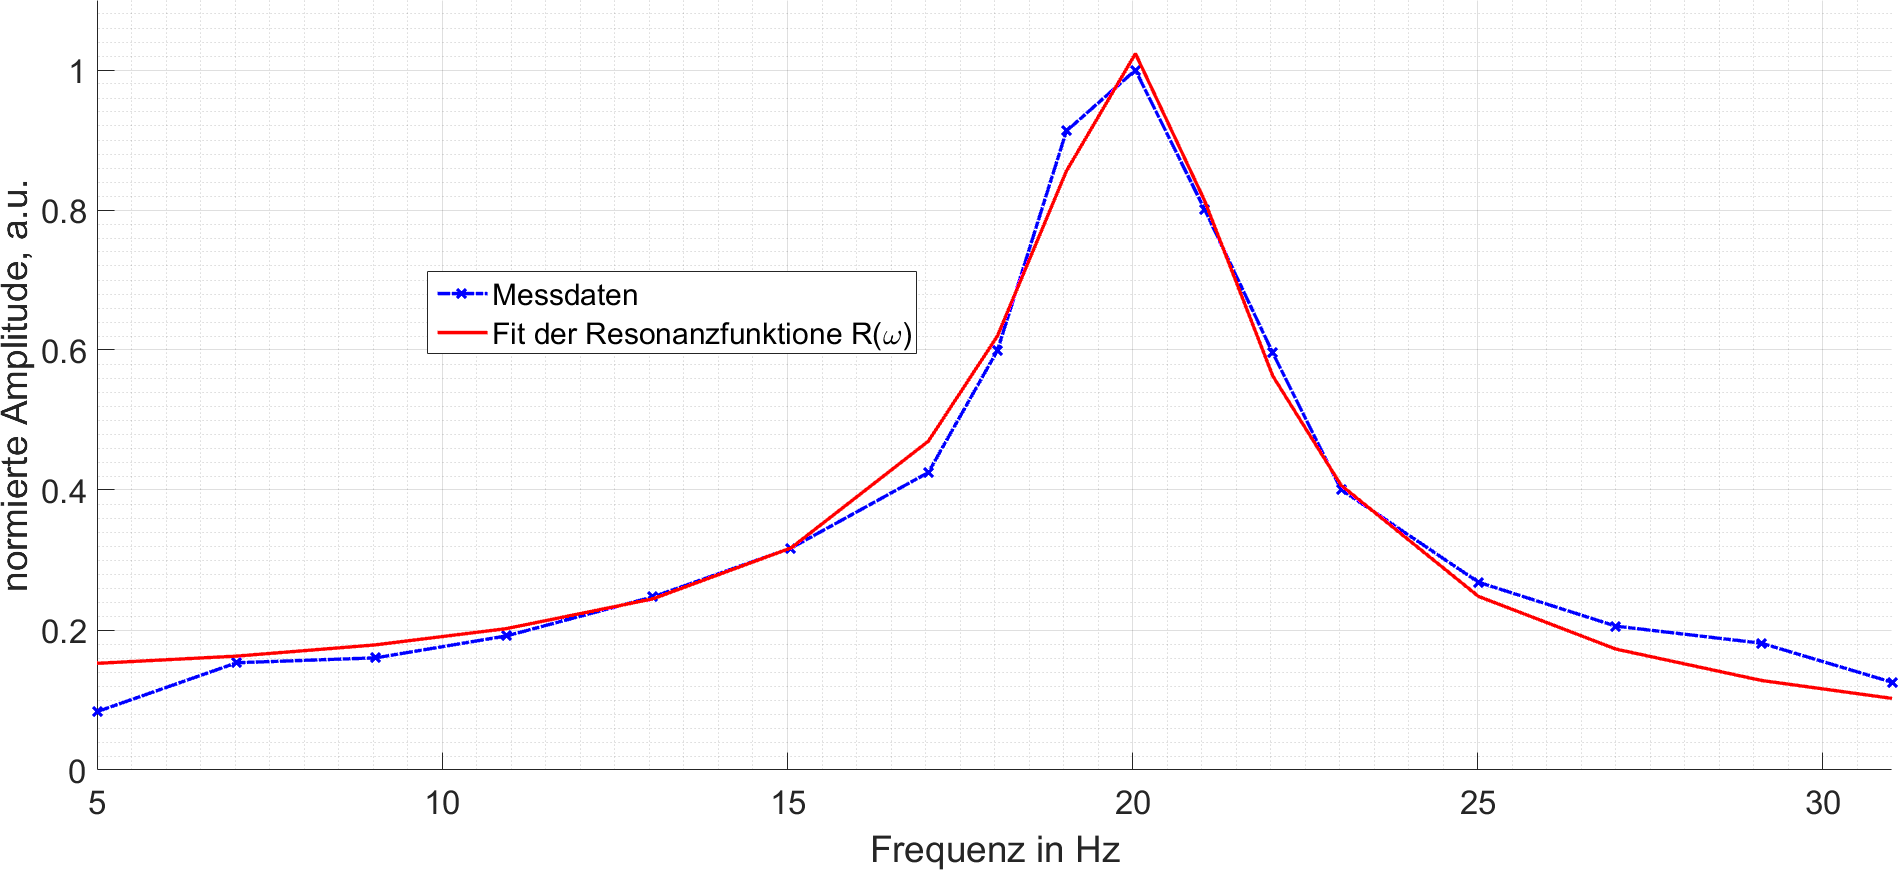
\includegraphics[width=\textwidth]{figs/res_schick.png}
			\caption{Resonanzantwort der 2D-Schicht von Teilchen bei externer Anregung über den Elektroden-bias. Fit der Resonanzfunktion \autoref{eq:res}.}\label{img:freq}
		\end{figure}

	\clearpage

		Der Reibungskoeffizient wurde zu $\beta=\unit[17,682]{1/s}$.	Die Resonanzfrequenz bzw. die Kreis-Resonanzfrequenz ergab sich als:

			\begin{align}
				f\ix{0}=\unit[20,088]{Hz} \quad \omega\ix{0}=\unit[126,22]{rad/s} \,\, .\label{eq:resfreq}
			\end{align}

		Mit der gegebene Dichte, dem Radius und $m\ix{S}=4/3\pi a^3\rho$ ergibt sich eine Masse zu $\unit[2,269\tenpo{-12}]{kg}$ je Teilchen. Bei einer Leistung von $\unit[7]{W}$ und einem Druck von $\approx\unit[15]{pa}$ erhält man aus \cite{EMAUGreifswaldPlasm} eine Elektronendichte im Plasma von $\approx\unit[0.7\tenpo{15}]{m^{-3}}$. Über \autoref{eq:konstfeld} und $n\ix{e}=\alpha n\ix{I}$ folgt damit eine Feldstärke in der Randschicht über der Elektrode von $\unit[4,152\tenpo{7}]{V/m}$.\\
		Über die Definition der Resonanzfrequenz $\omega\ix{0}^2=Q\ix{S}E\ix{1}/m\ix{s}$ ergibt sich letztendlich

			\begin{align}
				Q\ix{S}=\unit[8,71\tenpo{-16}]{Coul}\approx 5436\cdot e \label{eq:lad}
			\end{align}

	\subsection{Thermische Geschwindigkeit}

		Mit Hilfe der zur Verfügung gestellten Software \tilt{KristallAuswertung.m} wurde die mittlere Verschiebung der Teilchen von einem frame zum anderen in den Aufnahmen des 2. Versuchstages bestimmt. Wichtig dabei ist, dass nur 9 der ca. 21 Teilchen im System von der Software betrachtet wurden. Es wurde mit rund 60 fps für 1000 frames aufgenommen. \\
		Das Programm ermittelte eine Verschiebung von $\unit[0,99\pm 0.68]{px}$ pro Bild. Da der Fehler die Größenordnung des Ergebnisses hat, ist dieses Ergebnis zu hinterfragen.\\
		Mittels der Kalibration mit dem Millimeterpapier (siehe \autoref{img:milli}) erhielt man den Maßstab von $\unit[43,01]{px/mm}$. Damit wird die mittlere thermische Geschwindigkeit zu

			\begin{align}
				v\ix{th,S}=\unit[0,023]{mm/frame}=\unit[1,381]{mm/s} \,\, .\label{eq:geschw}
			\end{align}

		Zusammen mit dem, von der Software angegeben Fehler erhält man, dass der Wahre Wert $v\ix{th,true}$ im Intervall $\left[2,329; 0,4324\right]\unit{mm/s}$ liegen muss. Das Unterstreicht die Aussage von vorher wiederum, da die Intervalllänge etwa die Dimension des ersten Wertes hat.\\
		Im gleichen Zuge wie die Festlegung der Skalen, kann die Bestimmung des mittleren Teilchenabstandes $\overline{b}$ vorgenommen werden. Man erhält den Wert $\unit[0,795]{mm}$, woraus sich der Wigner-Seitz-Radius nach \autoref{eq:2dim} zu

			\begin{align}
				b\ix{WS}=\unit[0,739]{mm} \label{eq:wigner}
			\end{align}

		ergibt.\\
		Somit kennen wir alle wichtigen Größen des Systems. Damit können wir weitere Berechnungen anstellen: nach $v\ix{th,S}^2=8k\ix{B}T\ix{S}/(\pi m\ix{S})$ (analog \autoref{eq:elektronenstrom} usw.) bestimmt man die Staubtemperatur.

			\begin{align}
				T\ix{S}=\unit[123174]{K}\,\hat{=}\,\unit[10,61]{eV} \label{eq:temp}
			\end{align}

	\subsection{Kopplungsparameter und Fehlerbetrachtung}

		Da alle notwendigen Größen für die Berechnung von \autoref{eq:kopplung} nun bekannt sind, errechnet man leicht dessen Wert. Zusätzlich ist in \cite{EMAUGreifswaldPlasm} die Debye-Länge $\lambda\ix{D}=(525\pm25)\unit{\upmu m}$ gegeben.

			\begin{align}
				\Gamma=5,423\quad\Gamma\ix{C,eff}=1,326 \label{eq:koppwert}
			\end{align}

		Das spricht offensichtlich für ein stark gekoppeltes System, in welchem aber noch die thermische und elektrische Wechselwirkung die gleichen Dimensionen besitzen. Auch in Rückblick auf die Ladung bzw.die Ladungszahl scheinen die erhaltenen Größen realistisch. In derartigen Laborplasmen sind $\tenpo{2}\dots\tenpo{4}\cdot e$ gegeben. Auch die thermische Energie von $\approx\unit[10]{eV}$ ist im Rahmen der Experiment-Parameter eine gute Größe.\\
		Wählt man eine andere Herangehensweise an die Staubladung, nämlich über \autoref{eq:ladung}, so ergeben sich gänzlich andere Größen. Des Weiteren ist die Elektronendichte aus \cite{EMAUGreifswaldPlasm} bekannt, weswegen die dafür notwendige Elektronentemperatur bestimmt werden kann ($\approx0,61n\ix{e,0}$). Bezieht man außerdem noch das Fehlerintervall der Debye-Länge mit ein, so ergeben sich die folgenden Größen:

			\begin{align}
				T\ix{e}\in&\left[\unit[27130]{K}; \unit[22421]{K}\right] \nonumber\\
				Z\ix{S}\in&\left[23346; 19319\right] \nonumber\\
				\Gamma\in&\left[100,03; 68,5\right] \nonumber\\
				\Gamma\ix{C,eff}\in&\left[26,08; 15,61\right]\,\,. \nonumber
			\end{align}

		Im Hinblick auf die Kopplungsparameter und Staubtemperaturen erscheinen diese Ergebnisse sinnvoller, als die obigen. Der Wert von $\Gamma$ deutet eine sehr starke, aber noch keine kristalline Kopplung an. Der Effektiv-Wert repräsentiert das ebenfalls. Die Beobachtungen am System - schwache Amplituden, kleines thermisches Schwanken - stimmen mehr mit den neuen Größenintervallen überein, als die vorherigen. Das Modell des gedämpften, getriebenen harmonischen Oszillators als Staubteilchen kann also als ungenügend betrachtet werden.\\
		Für die benutzerdefinierte Eingaben kann man einen Fehler von $\pm\unit[2]{px}$ ansetzen.Die Abweichungen pflanzen sich folgendermaßen fort:

			\begin{align}
				b\ix{WS}\in&\left[\unit[0.781]{mm}; \unit[0.698]{mm}\right] \nonumber \\
				Z\ix{S}\in&\left[5831; 5012\right] \nonumber \\
				T\ix{S}\in&\left[\unit[9,68]{eV}; \unit[11,67]{eV}\right] \nonumber \\
				v\ix{th,S}\in&\left[\unit[1,319]{mm/s}; \unit[1,448]{mm/s}\right] \nonumber \\
				\Gamma\in&\left[5,624; 5,253\right] \nonumber \,\,.
			\end{align}

		Die Auswirkungen der Fehler in einer GUI sind allgemein gering. Sie verändern die Interpretationsmöglichkeiten der errechneten Werte nicht.\\
		Abschließend bleibt die Frage, ob und in welcher Ordnung ein Fehler in der Ermittlung von $\overline{b}$ und dem mittleren Schwankungsquadrat in \tilt{KristallAuswertung.m} vorliegt.

	\newpage
	\section{Anhang}

		\bibliography{all.bib}
		\bibliographystyle{unsrt}

\end{document}